\begin{appendices}

\chapter{Detailed acknowledgments}
\label{app:ack}
I would like to thank the following creators for providing their works in a open, free of charge form:
\begin{itemize}
	\item French Baguette (https://sketchfab.com/FrenchBaguette) for their Painterly Stone Bench model;
	\item memoryleakx (https://sketchfab.com/memoryleakx) for their Old Lantern model;
	\item RoboHoloclone12 (https://sketchfab.com/RoboHoloclone12) for their Park Trash Bin model;
	\item François Espagnet (https://sketchfab.com/francoisespagnet) for their Road sign - No entry model;
	\item filipeb2011 (https://sketchfab.com/filipeb2011) for their Old Sign Post model;
	\item Huargenn (https://sketchfab.com/Huargenn) for their Japanese stone lantern model;
	\item Renafox (https://sketchfab.com/kryik1023) for their SMZ S3D Cycle-Car model;
	\item BitGem (https://sketchfab.com/bitgem) for their Low Poly Hand Painted Dungeon Stone Pillar model;
	\item supaluci (https://sketchfab.com/supaluci) for their pillar model;
	\item deizeshot (https://sketchfab.com/deizeshot) for their De\_OldWall model;
	\item Inuciian (https://sketchfab.com/Inuciian) for their Wooden Window model;
	\item reymarch (https://sketchfab.com/reymarch) for their Low Poly Trees model;
	\item klangfabrik (https://freesound.org/people/klangfabrik/) for their TONE 100 Hz 44.1 16bit sound; % Source: https://freesound.org/people/klangfabrik/sounds/28638/
	\item FreqMan (https://freesound.org/people/FreqMan/) for their concrete blocks moving2 sound. % https://freesound.org/people/FreqMan/sounds/25846/
\end{itemize}

\chapter{Pilot 2: Spatial Judgment. Controls}
\label{app:pilot2_controls}
\begin{figure}[h]
	\centering
	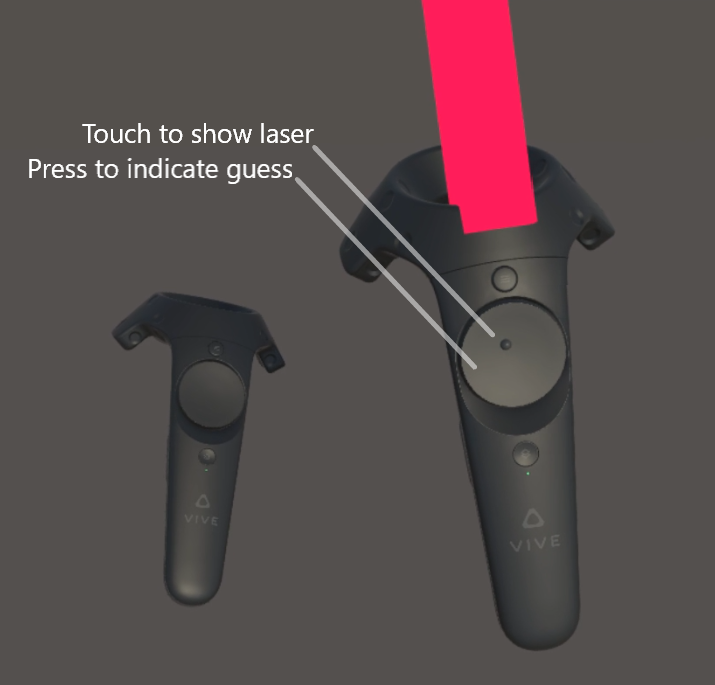
\includegraphics[width=0.7\linewidth]{figures/pilot2_tutorial_controllers_with_explanation}
	\caption{Controls}
	\label{fig:pilot2tutorialcontrollerswithexplanation}
\end{figure}

To indicate that translation started or ended at some point, participants would point the laser pointer at the wall and click the touchpad. They got a visual cue that they had made a selection (Fig. \ref{fig:pilot2tutorialgivinganswer}).

\begin{figure}
	\centering
	
	\subfloat{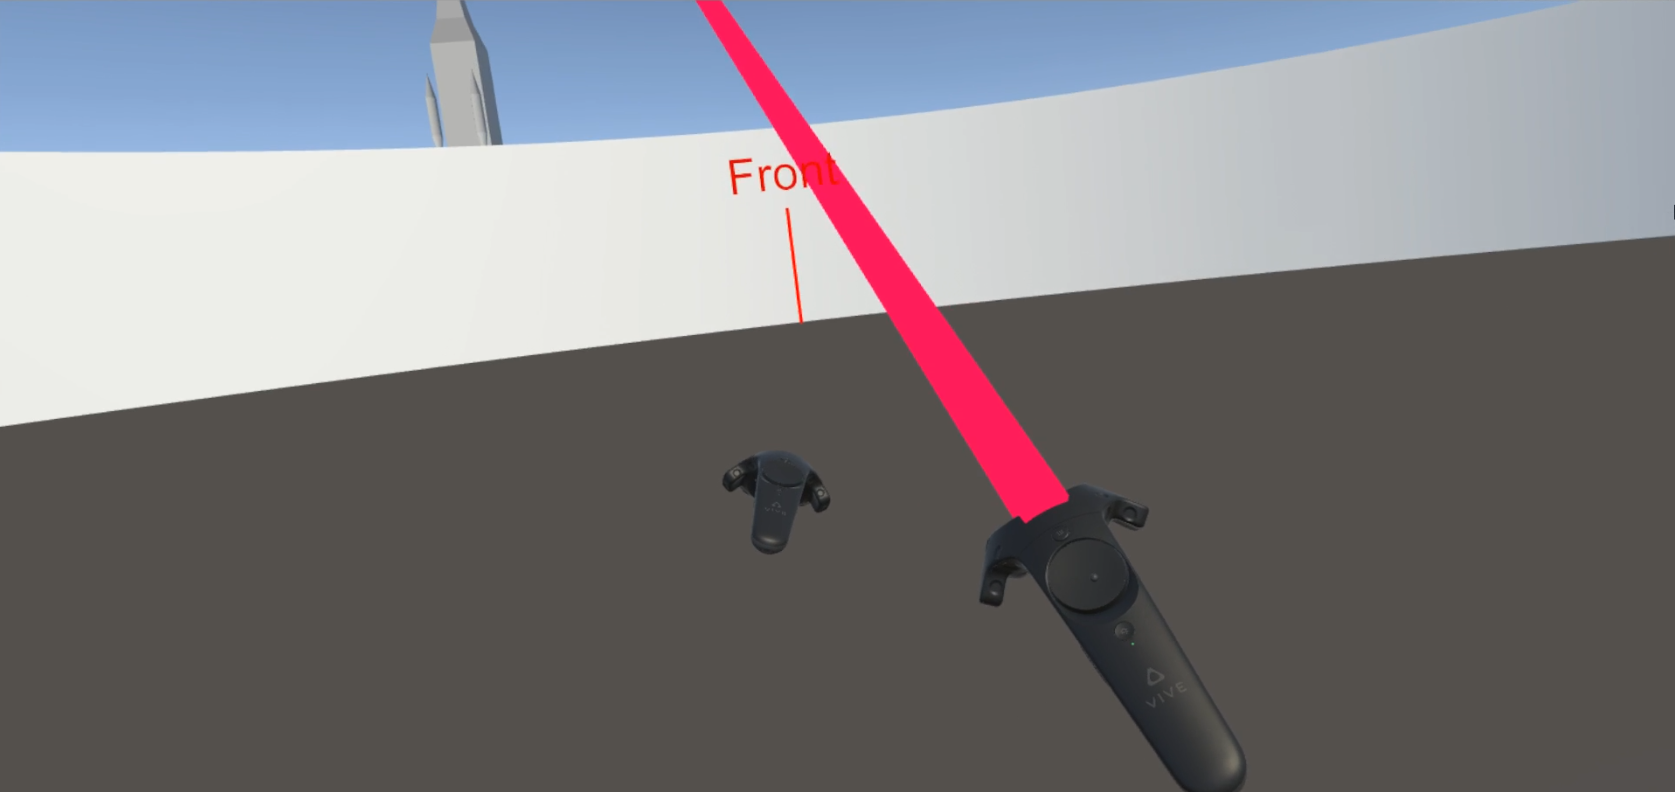
\includegraphics[width=0.7\linewidth]{figures/pilot2_tutorial_givinganswer1}}
	\par
	\subfloat{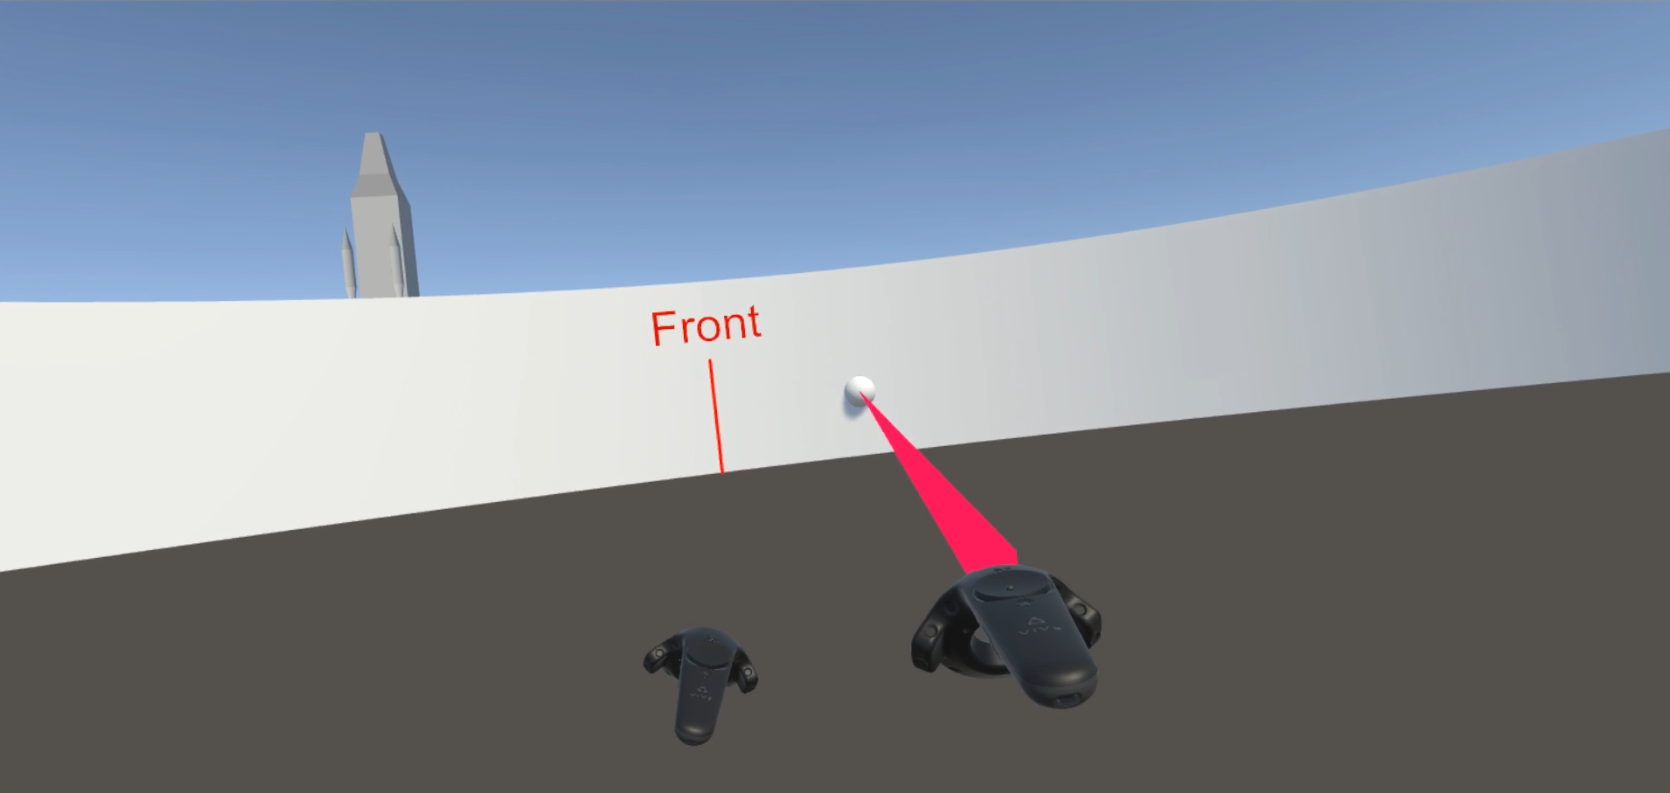
\includegraphics[width=0.7\linewidth]{figures/pilot2_tutorial_givinganswer2}}
	\par
	\subfloat{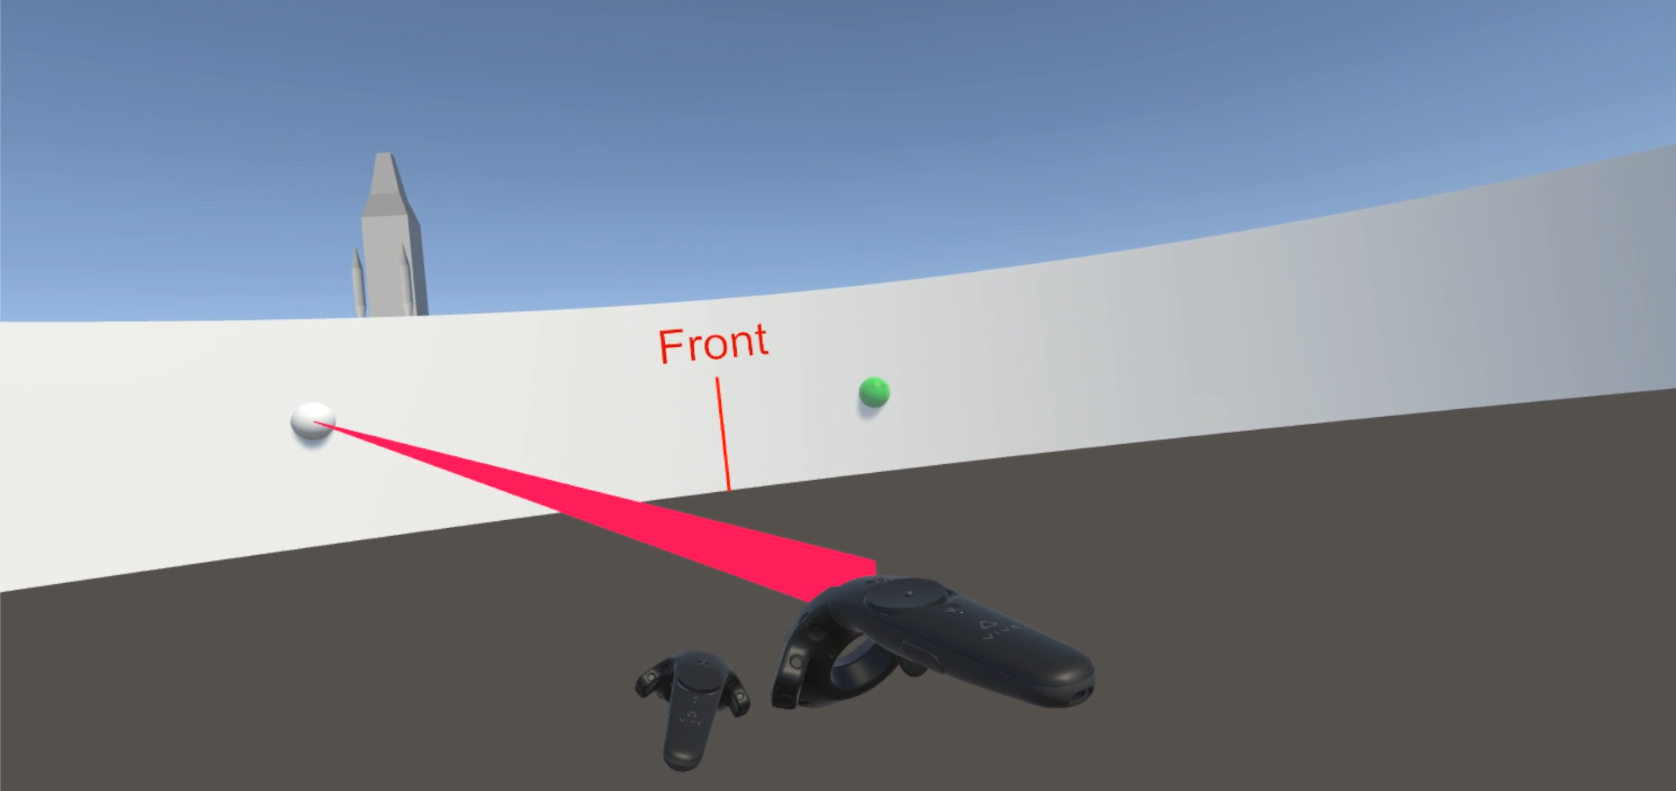
\includegraphics[width=0.7\linewidth]{figures/pilot2_tutorial_givinganswer3}}
	
	\caption{Giving an answer (a guess)}
	\label{fig:pilot2tutorialgivinganswer}
\end{figure}


\chapter{Pilot 2: Spatial Judgment. Questionnaire Data}
\label{app:pilot2questionnaire_data}

% \newline and \linebreak didn't work for the line break inside a cell	

\begin{table}[]
	\begin{tabularx}{\linewidth}{|X|l|l|X|X|X|}
		\hline
		\textbf{Participant num.} & \textbf{Gender} & \textbf{Age} & \textbf{Agree/Disagree: I have a good amount of experience in VR} & \textbf{A/D: I have good hearing} & \textbf{A/D: I am a regular online gamer} \\ \hline
		1                       & Male            & 23           & Strongly Agree                                                    & Agree                             & Agree                                     \\ \hline
		2                       & Male            & 29           & Strongly Agree                                                    & Strongly Agree                    & Neutral                                   \\ \hline
		3                       & Male            & 29           & Disagree                                                          & Strongly Agree                    & Strongly Disagree                         \\ \hline
		4                       & Male            & 30           & Strongly Agree                                                    & Disagree                          & Agree                                     \\ \hline
		5                       & Male            & 22           & Strongly Agree                                                    & Neutral                           & Disagree                                  \\ \hline
		6                       & Male            & 22           & Strongly Agree                                                    & Agree                             & Agree                                     \\ \hline
		7                       & Male            & 21           & Strongly Agree                                                    & Strongly Agree                    & Disagree                                  \\ \hline
		8                       & Female          & 20           & Agree                                                             & Neutral                           & Disagree                                  \\ \hline
		9                       & Female          & 24           & Strongly Agree                                                    & Agree                             & Agree                                     \\ \hline
		10                      & Female          & 32           & Disagree                                                          & Agree                             & Disagree                                  \\ \hline
		11                      & Female          & 50           & Agree                                                             & Disagree                          & Strongly Disagree                         \\ \hline
		12                      & Male            & 54           & Disagree                                                          & Neutral                           & Agree                                     \\ \hline
		13                      & Male            & 27           & Strongly Agree                                                    & Strongly Agree                    & Strongly Agree                            \\ \hline
	\end{tabularx}
\end{table}	


\chapter{Pilot 2: Spatial Judgment. Example of Data Collected per Participant}
\label{app:pilot2data_collected}
Complete data is available in the GitHub repository: \textit{https://github.com/bowlingforsoap/Master-Thesis-Experiments} (branch: data-viz, path: Assets/Resources/). Data is split participant-wise, so each actualTranslationsAndGuesses*.csv file contains 40 translations and guesses ("*" - integer user id).

\chapter{Pilot 2: Spatial Judgment. Visual Analysis}
\label{app:pilot2visual_analysis}

\begin{figure}
	%\centering
	\subfloat[B-F]{\includegraphics[scale=0.105]{../Studies/SpatialJudgements/Generated/B-F.png}}\hfill
	\subfloat[B-L]{\includegraphics[scale=0.105]{../Studies/SpatialJudgements/Generated/B-L.png}}
	\par\smallskip
	\subfloat[B-LF]{\includegraphics[scale=0.105]{../Studies/SpatialJudgements/Generated/B-LF.png}}\hfill
	\subfloat[B-R]{\includegraphics[scale=0.105]{../Studies/SpatialJudgements/Generated/B-R.png}}
\end{figure}
\begin{figure}	
	\subfloat[B-RF]{\includegraphics[scale=0.105]{../Studies/SpatialJudgements/Generated/B-RF.png}}\hfill
	\subfloat[F-B]{\includegraphics[scale=0.105]{../Studies/SpatialJudgements/Generated/F-B.png}}
	\par\smallskip
	\subfloat[F-L]{\includegraphics[scale=0.105]{../Studies/SpatialJudgements/Generated/F-L.png}}\hfill
	\subfloat[F-R]{\includegraphics[scale=0.105]{../Studies/SpatialJudgements/Generated/F-R.png}}
	\par\smallskip
\end{figure}
\begin{figure}
	\subfloat[L-B]{\includegraphics[scale=0.105]{../Studies/SpatialJudgements/Generated/L-B.png}}\hfill
	\subfloat[F-LB]{\includegraphics[scale=0.105]{../Studies/SpatialJudgements/Generated/F-LB.png}}
	\par\smallskip
	\subfloat[F-RB]{\includegraphics[scale=0.105]{../Studies/SpatialJudgements/Generated/F-RB.png}}\hfill
	\subfloat[L-F]{\includegraphics[scale=0.105]{../Studies/SpatialJudgements/Generated/L-F.png}}
\end{figure}
\begin{figure}
	%	\centering
	
	\subfloat[L-R]{\includegraphics[scale=0.105]{../Studies/SpatialJudgements/Generated/L-R.png}}\hfill
	\subfloat[L-RB]{\includegraphics[scale=0.105]{../Studies/SpatialJudgements/Generated/L-RB.png}}
	\par\smallskip
	\subfloat[L-RF]{\includegraphics[scale=0.105]{../Studies/SpatialJudgements/Generated/L-RF.png}}\hfill
	\subfloat[LB-F]{\includegraphics[scale=0.105]{../Studies/SpatialJudgements/Generated/LB-F.png}}
\end{figure}
\begin{figure}
	\subfloat[LB-LF]{\includegraphics[scale=0.105]{../Studies/SpatialJudgements/Generated/LB-LF.png}}\hfill
	\subfloat[LB-R]{\includegraphics[scale=0.105]{../Studies/SpatialJudgements/Generated/LB-R.png}}
	\par\smallskip
	\subfloat[LB-RB]{\includegraphics[scale=0.105]{../Studies/SpatialJudgements/Generated/LB-RB.png}}\hfill
	\subfloat[LB-RF]{\includegraphics[scale=0.105]{../Studies/SpatialJudgements/Generated/LB-RF.png}}
	\par\smallskip
\end{figure}
\begin{figure}
	\subfloat[LF-LB]{\includegraphics[scale=0.105]{../Studies/SpatialJudgements/Generated/LF-LB.png}}\hfill
	\subfloat[LF-B]{\includegraphics[scale=0.105]{../Studies/SpatialJudgements/Generated/LF-B.png}}
	\par\smallskip
	\subfloat[LF-R]{\includegraphics[scale=0.105]{../Studies/SpatialJudgements/Generated/LF-R.png}}\hfill
	\subfloat[LF-RB]{\includegraphics[scale=0.105]{../Studies/SpatialJudgements/Generated/LF-RB.png}}
\end{figure}
\begin{figure}
	\subfloat[LF-RF]{\includegraphics[scale=0.105]{../Studies/SpatialJudgements/Generated/LF-RF.png}}\hfill
	\subfloat[R-F]{\includegraphics[scale=0.105]{../Studies/SpatialJudgements/Generated/R-F.png}}
	\par\smallskip
	\subfloat[R-B]{\includegraphics[scale=0.105]{../Studies/SpatialJudgements/Generated/R-B.png}}\hfill
	\subfloat[R-L]{\includegraphics[scale=0.105]{../Studies/SpatialJudgements/Generated/R-L.png}}
\end{figure}
\begin{figure}
	\subfloat[R-LB]{\includegraphics[scale=0.105]{../Studies/SpatialJudgements/Generated/R-LB.png}}\hfill
	\subfloat[R-LF]{\includegraphics[scale=0.105]{../Studies/SpatialJudgements/Generated/R-LF.png}}
	\par\smallskip
	\subfloat[RB-F]{\includegraphics[scale=0.105]{../Studies/SpatialJudgements/Generated/RB-F.png}}\hfill
	\subfloat[RB-L]{\includegraphics[scale=0.105]{../Studies/SpatialJudgements/Generated/RB-L.png}}
\end{figure}
\begin{figure}
	\subfloat[RB-LB]{\includegraphics[scale=0.105]{../Studies/SpatialJudgements/Generated/RB-LB.png}}\hfill
	\subfloat[RB-LF]{\includegraphics[scale=0.105]{../Studies/SpatialJudgements/Generated/RB-LF.png}}
	\par\smallskip
	\subfloat[RF-B]{\includegraphics[scale=0.105]{../Studies/SpatialJudgements/Generated/RF-B.png}}\hfill
	\subfloat[RB-RF]{\includegraphics[scale=0.105]{../Studies/SpatialJudgements/Generated/RB-RF.png}}
\end{figure}
\begin{figure}
	\centering
	
	\subfloat[RF-L]{\includegraphics[scale=0.105]{../Studies/SpatialJudgements/Generated/RF-L.png}}\hfill
	\subfloat[RF-LB]{\includegraphics[scale=0.105]{../Studies/SpatialJudgements/Generated/RF-LB.png}}
	\par\smallskip
	\subfloat[RF-RB]{\includegraphics[scale=0.105]{../Studies/SpatialJudgements/Generated/RF-RB.png}}\hfill
	\subfloat[RF-LF]{\includegraphics[scale=0.105]{../Studies/SpatialJudgements/Generated/RF-LF.png}}
	%	\caption{Visual analysis of the results, pilot 2, pt.2}
	%	\label{fig:pilot2resltsanalysispt2}
\end{figure}

\chapter{\nameref{final_study}. Controls}
\label{app:finalstudy_controls}
\begin{figure}[h]
	\centering
	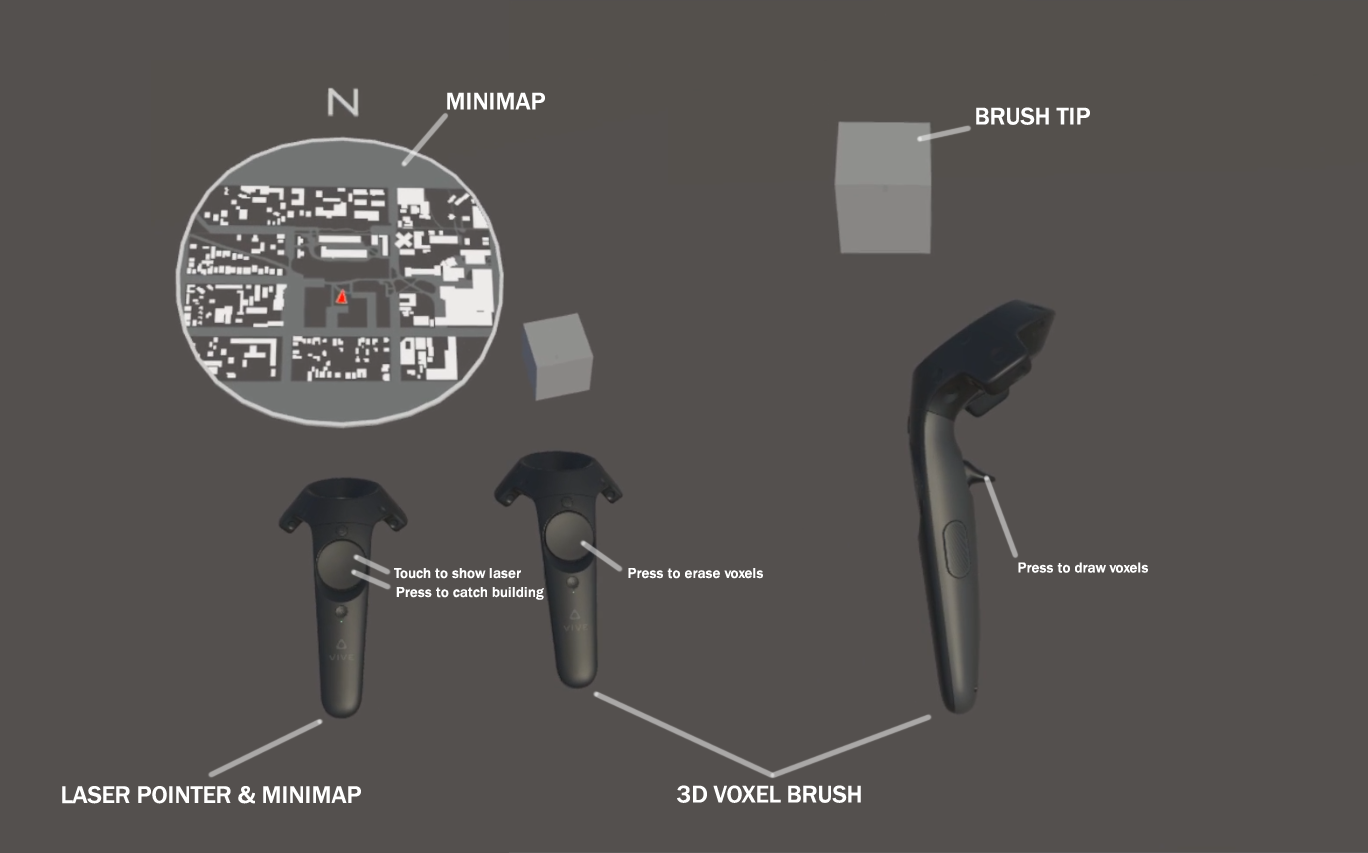
\includegraphics[width=\linewidth]{figures/finalstudy_controllers}
	\caption{Controls}
	\label{fig:finalstudycontrollers}
\end{figure}

To catch a moving building, user must point the laser pointer at the building and press the touch pad (Fig. \ref{fig:finalstudycatchingbuilding1}). Moving buildings are automatically supplied with a sphere collider that makes a raycasting volume bigger and the catching process easier. Additionally, it is possible to pinpoint the buildings that are behind other buildings in the scene.

\begin{figure}
	\centering
	
	\subfloat{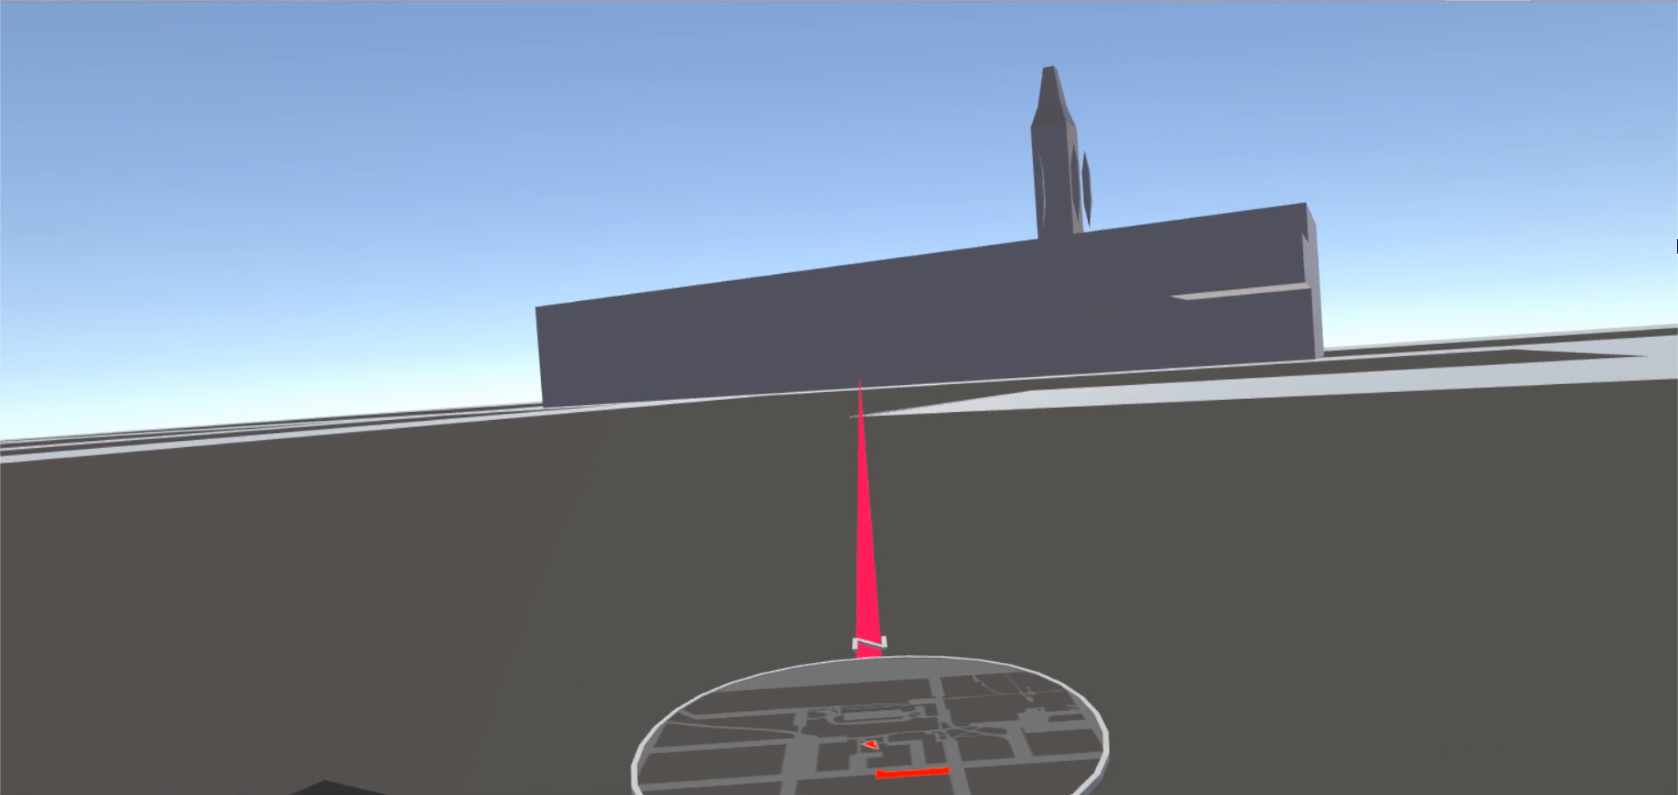
\includegraphics[width=0.7\linewidth]{figures/finalstudy_catchingbuilding1}}
	\par \smallskip
	\subfloat{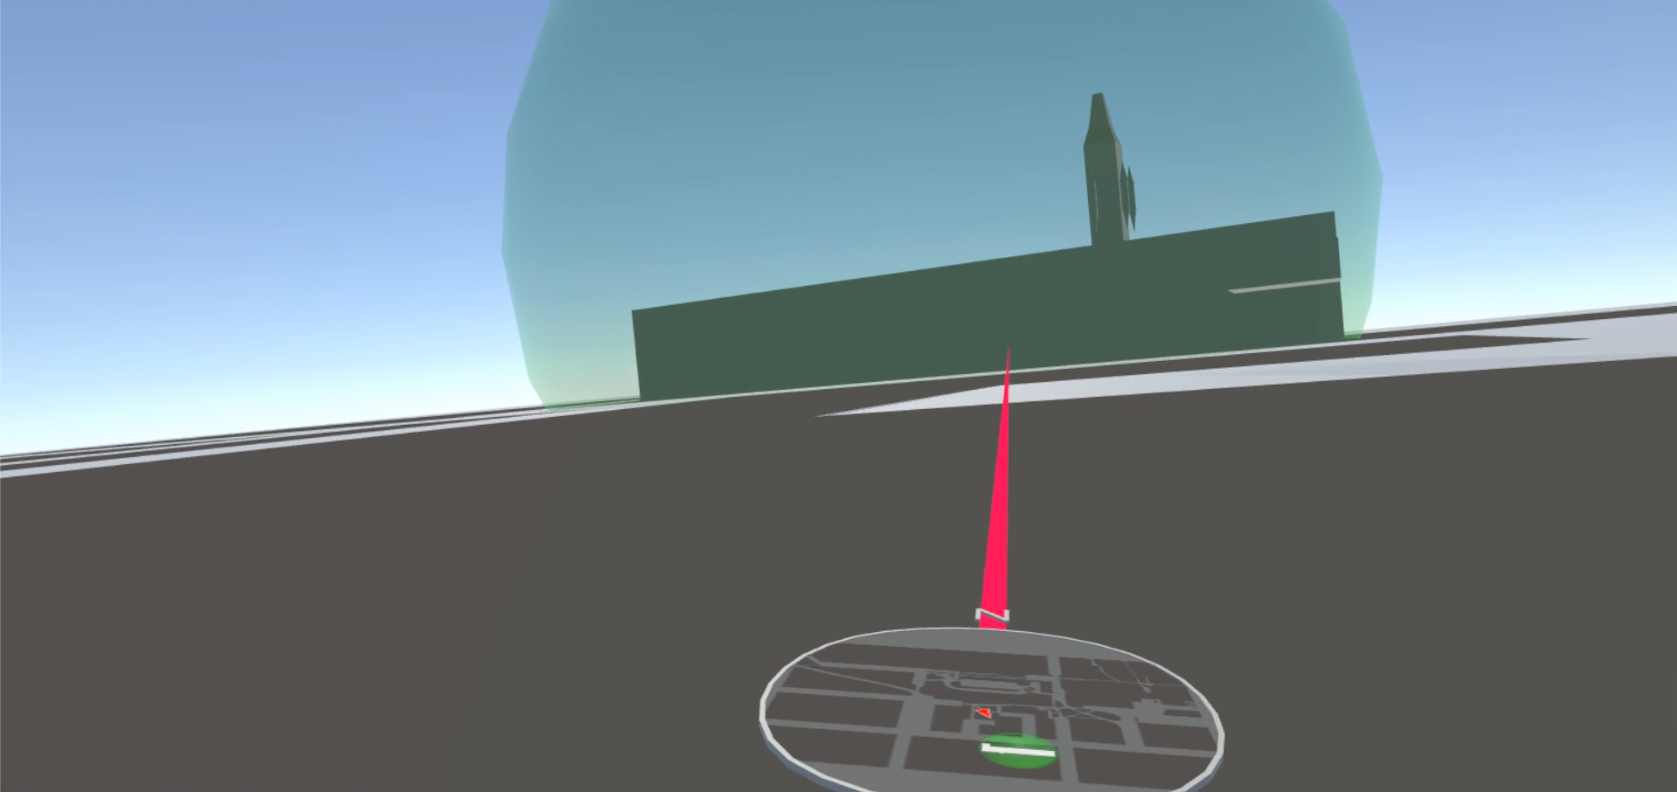
\includegraphics[width=0.7\linewidth]{figures/finalstudy_catchingbuilding2}}
	
	\caption{Catching a building}
	\label{fig:finalstudycatchingbuilding1}
\end{figure}


\chapter{\nameref{final_study}. Tracing Shapes}
\label{app:finalstudy_tracingshapes}

\begin{figure}
	\centering
	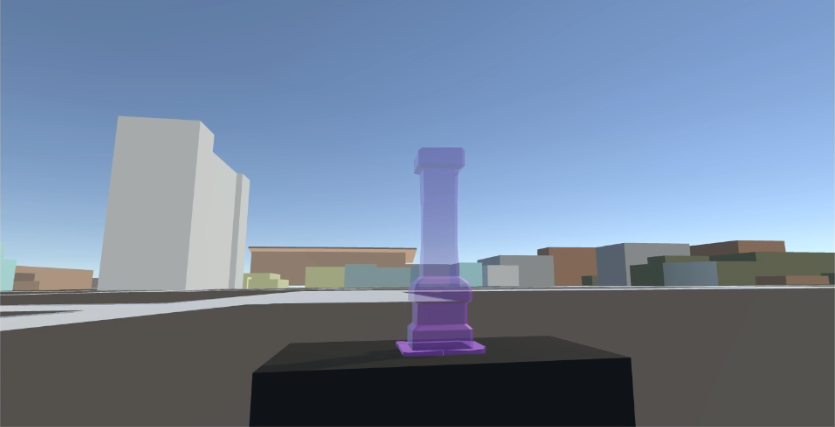
\includegraphics[width=0.9\linewidth]{figures/tracing_shapes/finalstudy_shapes1}
	\par \smallskip
	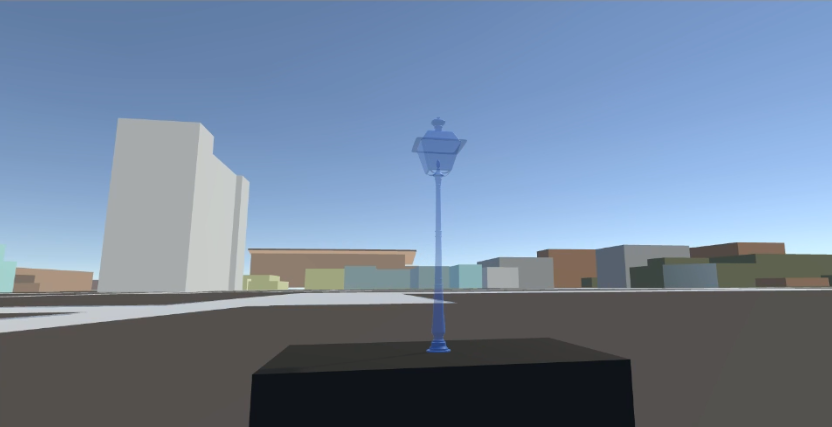
\includegraphics[width=0.9\linewidth]{figures/tracing_shapes/finalstudy_shapes2}
	\par \smallskip
	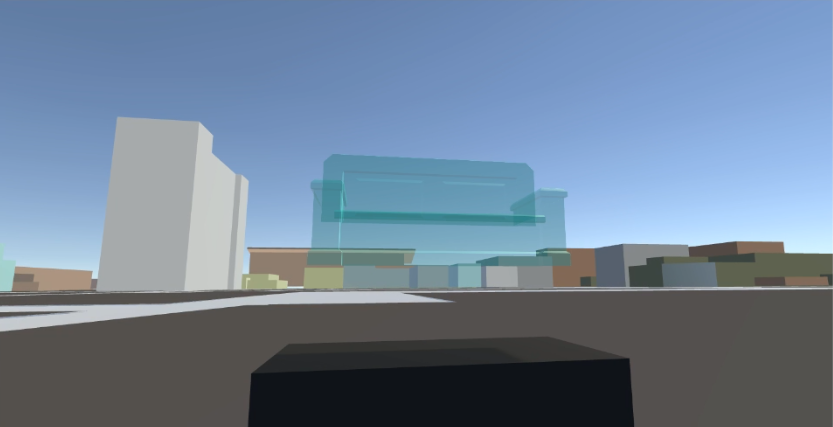
\includegraphics[width=0.9\linewidth]{figures/tracing_shapes/finalstudy_shapes3}
	\par \smallskip
\end{figure}
\begin{figure}
	\centering
	\includegraphics[width=0.9\linewidth]{figures/tracing_shapes/finalstudy_shapes4}
	\par \smallskip
	\includegraphics[width=0.9\linewidth]{figures/tracing_shapes/finalstudy_shapes5}
	\par \smallskip
	\includegraphics[width=0.9\linewidth]{figures/tracing_shapes/finalstudy_shapes6}
	\par \smallskip
\end{figure}
\begin{figure}
	\centering
	
	\includegraphics[width=0.9\linewidth]{figures/tracing_shapes/finalstudy_shapes7}
	\par \smallskip
	\includegraphics[width=0.9\linewidth]{figures/tracing_shapes/finalstudy_shapes8}
	\par \smallskip
	\includegraphics[width=0.9\linewidth]{figures/tracing_shapes/finalstudy_shapes9}
	\par \smallskip
\end{figure}
\begin{figure}
	\centering
	\includegraphics[width=0.9\linewidth]{figures/tracing_shapes/finalstudy_shapes10}
	\par \smallskip
	\includegraphics[width=0.9\linewidth]{figures/tracing_shapes/finalstudy_shapes11}
	\par \smallskip
	\includegraphics[width=0.9\linewidth]{figures/tracing_shapes/finalstudy_shapes12}
\end{figure}
\begin{figure}[t]
	\centering
	\includegraphics[width=0.9\linewidth]{figures/tracing_shapes/finalstudy_shapes13}
\end{figure}


\chapter{\nameref{final_study}. Data Collected}
\label{app:final_study_data_collected}
Complete data is available in the GitHub repository: \textit{https://github.com/bowlingforsoap/Master-Thesis-Experiments} (branch: workspace-awareness-study, path: Assets/Resources/). Data is stored in the \textit{workspace\_awareness\_study.csv} file. Alternatively, the same data, but in the Google Sheets format can be found at: \textit{https://preview.tinyurl.com/y94lc58x}.

\chapter{3D Voxel Drawings}
\label{app:3dDrawings}

\begin{figure}
	\centering
	\subfloat{\includegraphics[width=.8\linewidth]{figures/finalstudy_3DvoxelDrawings_2}}
	\par \smallskip
	\subfloat{\includegraphics[width=.8\linewidth]{figures/finalstudy_3DvoxelDrawings_3}}
	\par \smallskip
	\subfloat{\includegraphics[width=.8\linewidth]{figures/finalstudy_3DvoxelDrawings_1}}
\end{figure}


\chapter{\nameref{final_study}. Self-Report Questionnaire}
\label{app:final_study_questionnaire}
\includepdf[pages={1,2}]{D://Documents/studies/ss18/Thesis/Studies/WorkspaceAwareness/Questionnaire.pdf}

\end{appendices}